% ----------------------------------------------------------------
\section{Introduction}
\label{sec:introduction}

In this exercise, we are going to optimize \Gemm{} (General Matrix-Matrix
Multiplication) on modern computer architectures.
Specifically, we consider the simple case:
$$C:=C+A*B$$
where $A$, $B$, and $C$ are $n\times n$ matrices. \Gemm{} can be performed using
$2n^3$ floating point operations, as illustrated in the following pseudocode:





% ----------------------------------------------------------------
\section{The Goto Approach to Implementing {\sc gemm}}
\label{sec:BLIS}

\begin{figure}[tb!]
\begin{center}
\begin{minipage}{3in}
\mbox{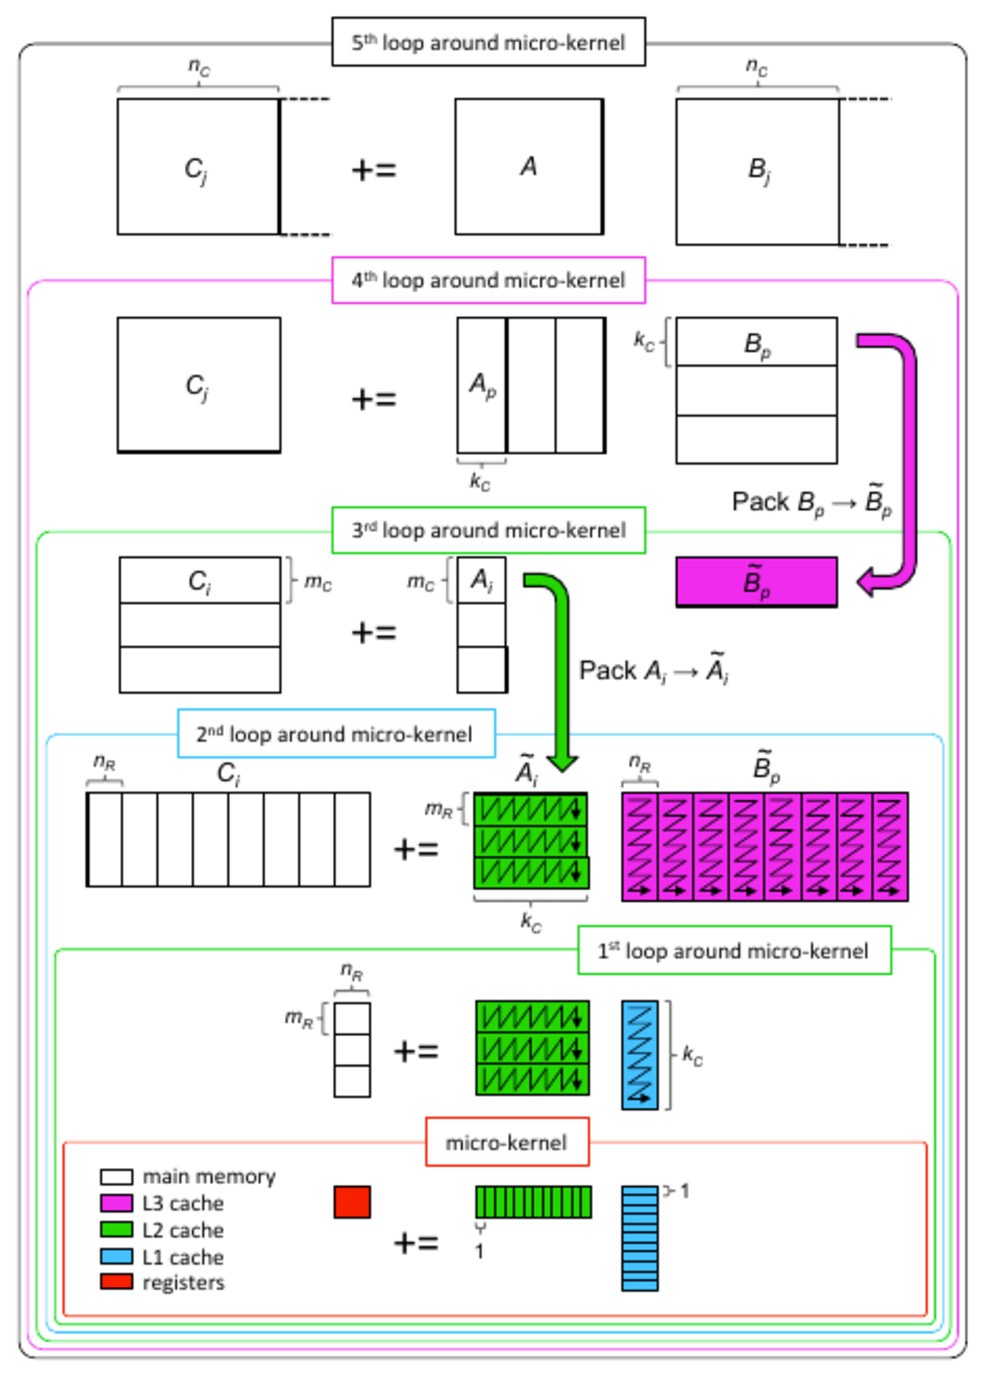
\includegraphics[width=3.0in]{mm_blis_color.pdf}}
\end{minipage}
~~~
\begin{minipage}[t]{3in}
\footnotesize  
\mbox{\input blis_gemm_new  }
\end{minipage}
\end{center}
\caption{Left: The Goto algorithm for matrix-matrix multiplication as  
  refactored in BLIS.  Right: the same algorithm, but expressed as  
  loops.}
\label{fig:blis_gemm}
\end{figure}

\cite{Goto:2008:AHP}
\cite{BLIS1}
\cite{BLIS2}
\cite{BLIS3}
\cite{BLIS4}



% ----------------------------------------------------------------
Architecture: Ivy Bridge and Haswell.

\section{Naive Approach: Three loops}



\section{Cache Blocking: 6 loops}

refer to GOTO paper: How to permuate to get the best loop order
var2, var1, var3


Performance Graph

\section{Add packing}


\section{Kernel Tricks}
1. Butterfly or Broadcasting?

2. Double buffering



\section{Parameter Tuning}




\section{Parallelization}










% ----------------------------------------------------------------
\section{Conclusion}
\label{sec:conclusion}

Conclusion.


\subsection*{Additional information}

For additional information on FLAME visit
\begin{center}
\href{http://www.cs.utexas.edu/users/flame/}
     {\tt http://www.cs.utexas.edu/users/flame/}.
\end{center}
